\chapter{Fundamentos}
    \label{chp:fundamentos}
    %\section{Revisão de Literatura} %Artigos sobre pendulo invertido dinâmico, bicleta, etc.
	%\section{Revisão teórica}
    
    Neste capitulo é realizada a revisão teórica necessária para o desenvolvimento da modelagem dos subsistemas do pendulo invertido dinâmico.
    
    Os atuadores do subsistema de angulo de esterço e do subsistema de tração são baseados em um motor de Corrente Contínua de ímã permanente, daqui em diante abreviado como motor CC. Além disso, o subsistema de tração possui um acoplamento entre roda e motor através de uma polia-correia. Logo, é necessário fazer um revisão das equações que regem o funcionamento dessas partes.
    
	\section{Motor elétrico CC de ímã Permanente} \label{sec:motorcc}

        Os motores CC de ímã permanente oferecem uma série de benefícios uteis para aplicações de baixa potência em relação aos motores CC com enrolamento de campo. Possuem construção mais simples, necessitam de menos espaço e o custo de produção pode ser inferior em alguns casos. O principal beneficio é que os ímãs não necessitam de excitação externa nem dissipam a potência correspondente para criar campos magnéticos na máquina. A limitações impostas pelos ímãs permanentes, como o risco de desmagnetização e baixa densidade de fluxo, vem sendo superadas com o desenvolvimento de novos materiais magnéticos. A Figura~\ref{img:circuito} mostra o circuito equivalente de um motor CC de ímã permanente~\cite{book:fitzgerald}.
        
        \begin{figure}[h]
            \centering
            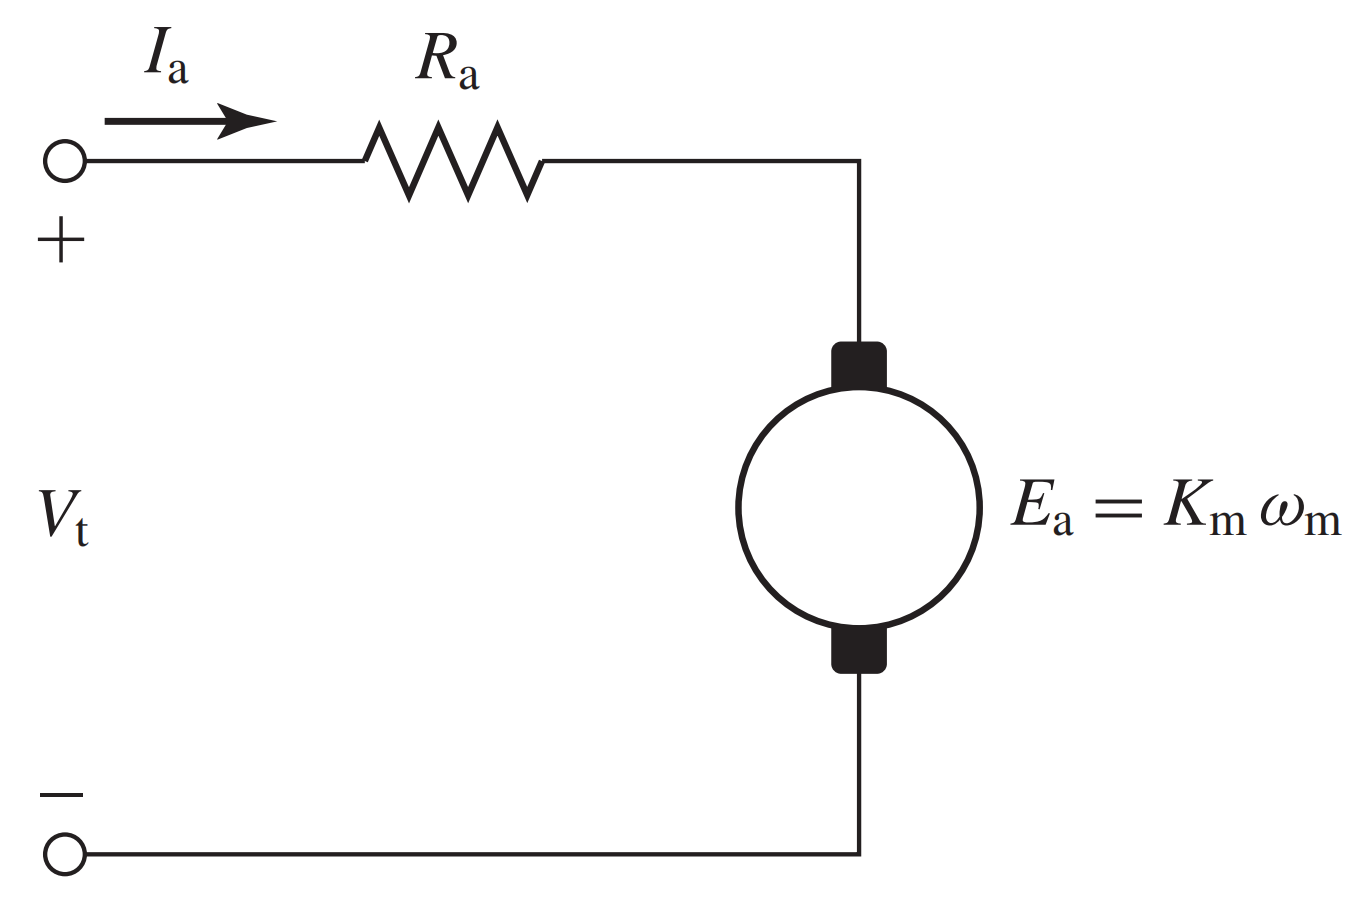
\includegraphics[width=10cm]{Imagens/Circuito_eq.png}
            \caption{Circuito equivalente de um motor CC com ímãs permanentes. Autoria de~\cite{book:fitzgerald}.}
            \label{img:circuito}
        \end{figure}
	    
	    A tensão gerada por um motor CC é descrita como
	    
		\begin{equation}
		    E_a = K_a \phi_d \omega_m ,
		    \label{eq:tensaoeletromotriz}
		\end{equation}
		%
		em que $K_a$ é a constante geométrica do motor, $\phi_d$ é o fluxo gerado pela ímã permanente, e $\omega_m$ é a velocidade angular do rotor do motor.
		
		Como o fluxo $\phi_d$ é constante, assim como a constante geométrica $K_a$, podemos criar uma nova constante, $K_m$, produto dessas duas a fim de simplificar as equações. Essa constante é chamada de "constante do motor". Assim,
		
		\begin{equation}
		    K_m = K_a \phi_d.
		\end{equation}
		
		Logo a Equação~\eqref{eq:tensaoeletromotriz} se torna
		
		\begin{equation}
            E_a = K_m \omega_m.
            \label{eq:tensaoeletromotrizsimplificada}
		\end{equation}
		
		O torque mecânico é dado pela expressão
		
		\begin{equation}
		    T_{mec} = \frac{E_a I_a}{\omega_m},
		\end{equation}
		%
		que pela Equação~\eqref{eq:tensaoeletromotrizsimplificada} se torna
		
		\begin{equation}
		    T_{mec} = K_m I_a.
		    \label{eq:torquemecanicosimplificado}
		\end{equation}
		
		Pelo circuito equivalente da Figura~\ref{img:circuito} temos que
		
		\begin{equation}
		    I_a = \frac{V_t - E_a}{R_a}.
		\end{equation}
		
		Substituindo $E_a$ pela expressão contida na Equação~\eqref{eq:tensaoeletromotrizsimplificada}, temos
		
		\begin{equation}
		    I_a = \frac{V_t - K_m \omega_m}{R_a}.
		\end{equation}
		
		E por fim, substituindo a expressão que relacionada $I_a$ com a tensão, na Equação~\eqref{eq:torquemecanicosimplificado}, é possível relacionar a o torque gerado com a tensão entrada e a velocidade angular do eixo
		
		\begin{equation}
		    T_{mec} = K_m \frac{V_t - K_m \omega_m}{R_a} = \frac{K_m}{R_a}V_t - \frac{K_m^2}{R_a}\omega_m.
		    \label{eq:torquemotor}
		\end{equation}
	
	\section{Modelagem e Identificação de Sistemas}
	
	    \subsection{Caixa Branca}
	    
	    \subsection{Caixa Preta}
	    
	    \subsection{Caixa Cinza}
	
	\section{Controladores do tipo PID}
	    
	    \subsection{Proporcional}
	    
	    %Lugar das raises
	    
	    \subsection{Proporcional e Integrativo}
	    
	    \subsection{Proporcional e Derivativo com Filtro}
	        
	        A função de transferência de um controlador PD é dada por:
	        
	        \begin{equation}
	            P_D(s) = K_p + s K_d 
	        \end{equation}
	        
	        Por ser uma função de transferência não causal, ou seja, o grau do numerador é maior que o do denominador, faz-se necessário adicionar pelo menos um polo ao controlador, de certa forma a pelo menos igualar o grau do numerador e denominador. Logo temos que:
	        
	        \begin{equation}
	            P_{DF}(s) = K_p + K_d \frac{sf}{s+f}
	            \label{eq:pdf}
	        \end{equation}
	        
	        Este polo atua como filtro do derivador, por isso ele será denominado de $f$.
	        
	        \subsection{Compensadores}
	  
    \section{Síntese de controladores PID: Síntese Direta}
	        %Referenciar CHEN
	
    \section{Espaço de estados}
    
    \section{Síntese de Controladores no Espaço de Estados: Alocação de Polos}

	
